  \documentclass[a4paper, 12pt]{book}
%\documentclass[a4paper, 12pt, draft]{book}  Nalogo preverite tudi z opcijo draft, ki vam bo pokazala, katere vrstice so predolge!
\usepackage[utf8x]{inputenc}   % omogoča uporabo slovenskih črk kodiranih v formatu UTF-8
\usepackage[slovene,english]{babel}    % naloži, med drugim, slovenske delilne vzorce
\usepackage[pdftex]{graphicx}  % omogoča vlaganje slik različnih formatov
\usepackage{fancyhdr}          % poskrbi, na primer, za glave strani
\usepackage{amssymb}           % dodatni simboli
\usepackage{amsmath}           % eqref, npr.
%\usepackage{hyperxmp}
\usepackage[hyphens]{url}  % dodal Solina
\usepackage{comment}       % dodal Solina
\usepackage{spverbatim}       % dodal Jakob
\usepackage[pdftex, colorlinks=true,
						citecolor=black, filecolor=black, 
						linkcolor=black, urlcolor=black,
						pagebackref=false, 
						pdfproducer={LaTeX}, pdfcreator={LaTeX}, hidelinks]{hyperref}
\usepackage{color}       % dodal Solina
\usepackage{soul}       % dodal Solina
%%%%%%%%%%%%%%%%%%%%%%%%%%%%%%%%%%%%%%%%
%	DIPLOMA INFO
%%%%%%%%%%%%%%%%%%%%%%%%%%%%%%%%%%%%%%%%
\newcommand{\ttitle}{Povezovanje Kubernetes gruč}
\newcommand{\ttitleEn}{Connecting Kubernetes clusters}
\newcommand{\tsubject}{\ttitle}
\newcommand{\tsubjectEn}{\ttitleEn}
\newcommand{\tauthor}{Jakob Hostnik}
\newcommand{\tkeywords}{gruča, oblak, Kubernetes, računalniška gruča, povezovanje gruč, mreža gruč, GitOps}
\newcommand{\tkeywordsEn}{cluster, cloud, Kubernetes, computer cluster, connecting clusters, cluster mesh, GitOps}
%%%%%%%%%%%%%%%%%%%%%%%%%%%%%%%%%%%%%%%%
%	HYPERREF SETUP
%%%%%%%%%%%%%%%%%%%%%%%%%%%%%%%%%%%%%%%%
\hypersetup{pdftitle={\ttitle}}
\hypersetup{pdfsubject=\ttitleEn}
\hypersetup{pdfauthor={\tauthor, jakob@hostnik.si}}
\hypersetup{pdfkeywords=\tkeywordsEn}
%%%%%%%%%%%%%%%%%%%%%%%%%%%%%%%%%%%%%%%%
% postavitev strani
%%%%%%%%%%%%%%%%%%%%%%%%%%%%%%%%%%%%%%%%  
\addtolength{\marginparwidth}{-20pt} % robovi za tisk
\addtolength{\oddsidemargin}{40pt}
\addtolength{\evensidemargin}{-40pt}
\renewcommand{\baselinestretch}{1.3} % ustrezen razmik med vrsticami
\setlength{\headheight}{15pt}        % potreben prostor na vrhu
\renewcommand{\chaptermark}[1]%
{\markboth{\MakeUppercase{\thechapter.\ #1}}{}} \renewcommand{\sectionmark}[1]%
{\markright{\MakeUppercase{\thesection.\ #1}}} \renewcommand{\headrulewidth}{0.5pt} \renewcommand{\footrulewidth}{0pt}
\fancyhf{}
\fancyhead[LE,RO]{\sl \thepage} 
%\fancyhead[LO]{\sl \rightmark} \fancyhead[RE]{\sl \leftmark}
\fancyhead[RE]{\sc \tauthor}              % dodal Solina
\fancyhead[LO]{\sc Diplomska naloga}     % dodal Solina
\newcommand{\BibTeX}{{\sc Bib}\TeX}
%%%%%%%%%%%%%%%%%%%%%%%%%%%%%%%%%%%%%%%%
% naslovi
%%%%%%%%%%%%%%%%%%%%%%%%%%%%%%%%%%%%%%%%  
\newcommand{\autfont}{\Large}
\newcommand{\titfont}{\LARGE\bf}
\newcommand{\clearemptydoublepage}{\newpage{\pagestyle{empty}\cleardoublepage}}
\setcounter{tocdepth}{1}	      % globina kazala
%%%%%%%%%%%%%%%%%%%%%%%%%%%%%%%%%%%%%%%%
% konstrukti
%%%%%%%%%%%%%%%%%%%%%%%%%%%%%%%%%%%%%%%%  
\newtheorem{izrek}{Izrek}[chapter]
\newtheorem{trditev}{Trditev}[izrek]
\newenvironment{dokaz}{\emph{Dokaz.}\ }{\hspace{\fill}{$\Box$}}
%%%%%%%%%%%%%%%%%%%%%%%%%%%%%%%%%%%%%%%%%%%%%%%%%%%%%%%%%%%%%%%%%%%%%%%%%%%%%%%
%% PDF-A
%%%%%%%%%%%%%%%%%%%%%%%%%%%%%%%%%%%%%%%%%%%%%%%%%%%%%%%%%%%%%%%%%%%%%%%%%%%%%%%
%%%%%%%%%%%%%%%%%%%%%%%%%%%%%%%%%%%%%%%% 
% define medatata
%%%%%%%%%%%%%%%%%%%%%%%%%%%%%%%%%%%%%%%% 
\def\Title{\ttitle}
\def\Author{\tauthor, jakob@hostnik.si}
\def\Subject{\ttitleEn}
\def\Keywords{\tkeywordsEn}
%%%%%%%%%%%%%%%%%%%%%%%%%%%%%%%%%%%%%%%% 
% \convertDate converts D:20080419103507+02'00' to 2008-04-19T10:35:07+02:00
%%%%%%%%%%%%%%%%%%%%%%%%%%%%%%%%%%%%%%%% 
\def\convertDate{%
    \getYear
}
{\catcode`\D=12
 \gdef\getYear D:#1#2#3#4{\edef\xYear{#1#2#3#4}\getMonth}
}
\def\getMonth#1#2{\edef\xMonth{#1#2}\getDay}
\def\getDay#1#2{\edef\xDay{#1#2}\getHour}
\def\getHour#1#2{\edef\xHour{#1#2}\getMin}
\def\getMin#1#2{\edef\xMin{#1#2}\getSec}
\def\getSec#1#2{\edef\xSec{#1#2}\getTZh}
\def\getTZh +#1#2{\edef\xTZh{#1#2}\getTZm}
\def\getTZm '#1#2'{%
    \edef\xTZm{#1#2}%
    \edef\convDate{\xYear-\xMonth-\xDay T\xHour:\xMin:\xSec+\xTZh:\xTZm}%
}
\expandafter\convertDate\pdfcreationdate 
%%%%%%%%%%%%%%%%%%%%%%%%%%%%%%%%%%%%%%%%
% get pdftex version string
%%%%%%%%%%%%%%%%%%%%%%%%%%%%%%%%%%%%%%%% 
\newcount\countA
\countA=\pdftexversion
\advance \countA by -100
\def\pdftexVersionStr{pdfTeX-1.\the\countA.\pdftexrevision}
%%%%%%%%%%%%%%%%%%%%%%%%%%%%%%%%%%%%%%%%
% XMP data
%%%%%%%%%%%%%%%%%%%%%%%%%%%%%%%%%%%%%%%%  
\usepackage{xmpincl}
\includexmp{pdfa-1b}
%%%%%%%%%%%%%%%%%%%%%%%%%%%%%%%%%%%%%%%%
% pdfInfo
%%%%%%%%%%%%%%%%%%%%%%%%%%%%%%%%%%%%%%%%  
\pdfinfo{%
    /Title    (\ttitle)
    /Author   (\tauthor, jakob@hostnik.si)
    /Subject  (\ttitleEn)
    /Keywords (\tkeywordsEn)
    /ModDate  (\pdfcreationdate)
    /Trapped  /False
}
%%%%%%%%%%%%%%%%%%%%%%%%%%%%%%%%%%%%%%%%%%%%%%%%%%%%%%%%%%%%%%%%%%%%%%%%%%%%%%%
%%%%%%%%%%%%%%%%%%%%%%%%%%%%%%%%%%%%%%%%%%%%%%%%%%%%%%%%%%%%%%%%%%%%%%%%%%%%%%%
\begin{document}
\selectlanguage{slovene}
\frontmatter
\setcounter{page}{1} %
\renewcommand{\thepage}{}       % preprecimo težave s številkami strani v kazalu
\newcommand{\sn}[1]{"`#1"'}                    % dodal Solina (slovenski narekovaji)
%%%%%%%%%%%%%%%%%%%%%%%%%%%%%%%%%%%%%%%%
%naslovnica
 \thispagestyle{empty}%
   \begin{center}
    {\large\sc Univerza v Ljubljani\\%
      Fakulteta za računalništvo in informatiko\\%
      Fakulteta za matematiko in fiziko}%
    \vskip 10em%
    {\autfont \tauthor\par}%
    {\titfont \ttitle \par}%
    {\vskip 3em \textsc{DIPLOMSKO DELO\\[5mm]        
    INTERDISCIPLINARNI UNIVERZITETNI\\ ŠTUDIJSKI PROGRAM PRVE STOPNJE\\ RAČUNALNIŠTVO IN MATEMATIKA}\par}%
    \vfill\null%
    {\large \textsc{Mentor}: izr. prof. dr. Mojca Ciglarič \par}%
   {\large \textsc{Somentor}:  asist. dr. Matjaž Pančur \par}%
    {\vskip 2em \large Ljubljana, 2021 \par}%
\end{center}
% prazna stran
%\clearemptydoublepage      % dodal Solina (izjava o licencah itd. se izpiše na hrbtni strani naslovnice)
%%%%%%%%%%%%%%%%%%%%%%%%%%%%%%%%%%%%%%%%
%copyright stran
\thispagestyle{empty}
\vspace*{8cm}
\noindent
{\sc Copyright}. 
Rezultati diplomske naloge so intelektualna lastnina avtorja in Fakultete za računalništvo in informatiko Univerze v Ljubljani.
Za objavo in koriščenje rezultatov diplomske naloge je potrebno pisno privoljenje avtorja, Fakultete za računalništvo in informatiko ter mentorja.
\begin{center}
\mbox{}\vfill
\emph{Besedilo je oblikovano z urejevalnikom besedil \LaTeX.}
\end{center}
% prazna stran
\clearemptydoublepage
%%%%%%%%%%%%%%%%%%%%%%%%%%%%%%%%%%%%%%%%
% stran 3 med uvodnimi listi
\thispagestyle{empty}
\vspace*{4cm}
\noindent
Fakulteta za računalništvo in informatiko izdaja naslednjo nalogo:
\medskip
\begin{tabbing}
\hspace{32mm}\= \hspace{6cm} \= \kill
Tematika naloge:
\end{tabbing}
TODO
Besedilo teme diplomskega dela študent prepiše iz študijskega informacijskega sistema, kamor ga je vnesel mentor. V nekaj stavkih bo opisal, kaj pričakuje od kandidatovega diplomskega dela. Kaj so cilji, kakšne metode uporabiti, morda bo zapisal tudi ključno literaturo.
\vspace{15mm}
\vspace{2cm}
% prazna stran
\clearemptydoublepage
% zahvala
\thispagestyle{empty}\mbox{}\vfill\null\it%
\noindent
Na tem mestu bi se zahvalil mentorici izr. prof. dr. Mojci Ciglarič za pripravljenost in mentorstvo.
Zahvalil bi se tudi somentorju asist. dr. Matjažu Pančurju za vse nasvete in pomoč pri pisanju diplomske naloge.
Zahvala pa gre tudi moji ženi, staršem, bratom, sestram in prijateljem za podporo in spodbudo pri študiju.
\rm\normalfont
% prazna stran
\clearemptydoublepage
%%%%%%%%%%%%%%%%%%%%%%%%%%%%%%%%%%%%%%%%
% posvetilo, če sama zahvala ne zadošča :-)
\thispagestyle{empty}\mbox{}{\vskip0.20\textheight}\mbox{}\hfill\begin{minipage}{0.55\textwidth}%
Mami Lučki.
\normalfont\end{minipage}
% prazna stran
\clearemptydoublepage
%%%%%%%%%%%%%%%%%%%%%%%%%%%%%%%%%%%%%%%%
% kazalo
\pagestyle{empty}
\def\thepage{}% preprecimo tezave s stevilkami strani v kazalu
\tableofcontents{}
% prazna stran
\clearemptydoublepage
%%%%%%%%%%%%%%%%%%%%%%%%%%%%%%%%%%%%%%%%
% seznam kratic
\chapter*{Seznam uporabljenih kratic}  % spremenil Solina, da predolge vrstice ne gredo preko desnega roba
\noindent\begin{tabular}{p{0.1\textwidth}|p{.4\textwidth}|p{.4\textwidth}}    % po potrebi razširi prvo kolono tabele na račun drugih dveh!
  {\bf kratica} & {\bf angleško}                             & {\bf slovensko} \\ \hline
  {\bf CRD} & custom resource definition & definicija tipov po meri \\
  {\bf DNS} & domain name system & sistem domenskih imen \\
  {\bf IP} & internet protocol & internetni protokol \\
  {\bf HA} & high availability & visoka razpoložljivost \\
  {\bf GA} & general availability & splošna dostopnost \\
  {\bf VPN} & virtual private network & navidezno zasebno omrežje \\
\end{tabular}
% prazna stran
\clearemptydoublepage
%%%%%%%%%%%%%%%%%%%%%%%%%%%%%%%%%%%%%%%%
% povzetek
\addcontentsline{toc}{chapter}{Povzetek}
\chapter*{Povzetek}
\noindent\textbf{Naslov:} \ttitle
\bigskip

\noindent\textbf{Avtor:} \tauthor
\bigskip
%\noindent\textbf{Povzetek:} 
\noindent 

Več računalnikov povezujemo v skupine predvsem zaradi zagotavljanja večje zmogljivosti in stabilnosti.
V zadnjih letih je bil na tem področju narejen zelo velik napredek in razvoj.
Tako je nastal tudi sistem Kubernetes, ki je zaradi svoje popularnosti postal de facto standard za upravljanje gruč in orkestracijo kontejnerjev.
A zelo pogosto ena sama računalniška gruča ni dovolj.
To se zgodi v primerih, ko imamo težave z dragim prenosom podatkov, preveliko latenco do naših uporabnikov ali pa  želimo še bolj povečati stabilnost ali varnost našega sistema.
Primerov uporabe je veliko in v diplomski nalogi si bomo pogledali nekaj najpogostejših.
Pogledali si bomo, ozadje povezovanja gruč in kakšne pristope lahko uporabimo za reševanje naših problemov.
Lotili se bomo implementacije in reševanja problemov skozi nekaj primerov uporabe na konktretnih problemih.
Poseben poudarek pa bomo dali tudi sinhronizaciji podatkov, saj je to eden zahtevnejših delov pri upravljanju več računalniških gruč.
Ugotovimo, da nam lahko sodobne metode povezovanja gruč zelo olajšajo njihovo upravljanje in preprosto rešijo tudi zahtevnejše probleme sinhronizacije podatkov.


\bigskip
\noindent\textbf{Ključne besede:} \tkeywords.
% prazna stran
\clearemptydoublepage
%%%%%%%%%%%%%%%%%%%%%%%%%%%%%%%%%%%%%%%%
% abstract
\selectlanguage{english}
\addcontentsline{toc}{chapter}{Abstract}
\chapter*{Abstract}
\noindent\textbf{Title:} \ttitleEn
\bigskip

\noindent\textbf{Author:} \tauthor
\bigskip
%\noindent\textbf{Abstract:} 
\noindent 

We connect more computers into groups mainly to ensure greater performance and stability.
in recent years, great progress and development have been made in this area.
This is how the Kubernetes system was created, which due to its popularity became a world standard for cluster management in container orchestration.
But very often a single computer cluster is not enough.
This happens in cases where we have problems with expensive data transfer, too much latency to our users, or we want to further increase the stability or security of our system.
There are many examples of use, and we will look at some of the most common ones in this degree paper.
We will look at the background of connecting clusters and what approaches we can use to solve our problems.
We will tackle implementation and problem-solving through some common real-world problems.
Furthermore, we will also place special emphasis on data synchronization, as this is one of the more difficult parts of managing multiple computer clusters.
We find that modern methods of connecting clusters can greatly facilitate their management and easily solve even more difficult data synchronization problems.

\bigskip
\noindent\textbf{Keywords:} \tkeywordsEn.
\selectlanguage{slovene}
% prazna stran
\clearemptydoublepage
%%%%%%%%%%%%%%%%%%%%%%%%%%%%%%%%%%%%%%%%
\mainmatter
\setcounter{page}{1}
\pagestyle{fancy}
\chapter{Uvod}
\label{uvod}
\section{Motivacija}
Glede orkestracije kontejnerjev je bil v zadnjih nekaj letih narejen zelo velik preboj. 
V postopku tega preboja se je razvil tudi Kubernetes API, ki je na tem področju rešil marsikatero težavo.
Kubernetes  je univerzalni način, ki nam omogoča, da več računalnikov povežemo v gručo, ki deluje kot ena samostojna enota. 
To reši marsikatero težavo v računalništvu in vsaj teoretično je to dovolj, da imamo visoko razpoložljivost (HA) naših storitev ~\cite{mastering-Kubernetes} in sinhrono delovanje več računalnikov.
A industrija je zelo hitro ugotovila, da obstaja kar nekaj primerov, ko ni dovolj, da ena skupina računalnikov deluje kot celota, ampak bi želeli med seboj povezati tudi te skupine.
Ta problem se je do sedaj reševalo na več različnih načinov.
So pa v zadnjem času tudi razvijalci Kubernetesa začeli bolj celostno reševati problem.
Poizkusili so problem rešiti s projektom Federation 1, zdaj pa se zdi, da bo Federation 2 oziroma KubeFed uspešno prešel iz alfa verzije v beta.
Skratka, v računalništvi je na tem področju zelo veliko zanimanja in razvoja.
\section{Cilj in vsebina naloge}
V tem diplomskem delu si bomo pogledali nekaj o reševanju problema povezovanja računalniških gruč, Kubernetesu in primere uporabe, ki izvirajo iz potreb industrije. 
Za vsakega od primerov si bomo pogledali kako se ta problem rešuje v Kubernetes okolju z uporabo orodja KubeFed in kako bi sinhronizirali tudi podatke.
\subsection{Prevelika latenca}
Ko spletne aplikacije postanejo bolj globalne zelo hitro opazimo, da uporabniki, ki so na drugi celini kot naši strežniki, preživijo veliko več časa pred ikonami za nalaganje, saj podatki do njih potujejo dalj časa.
Ta problem je rešljiv na način, da postavimo še eno gručo bližje naših uporabnikov.
Na primer eno gručo na celino.
Tu pa zelo pogosto želimo, da se podatki sinhronizirajo.
Zavedati se moramo, da strežniki v gruči zelo veliko komunicirajo, zato je priporočljivo, da so tudi v istem omrežju znotraj istega podatkovnega centra, saj se s tem ponavadi izognemo latenci. 
Prevelika latenca med vozlišči je tudi ena izmed glavnih omejitev, da ne moremo vseh vozlišč povezati v eno večjo gručo.
\begin{figure}[h]
\begin{center}
  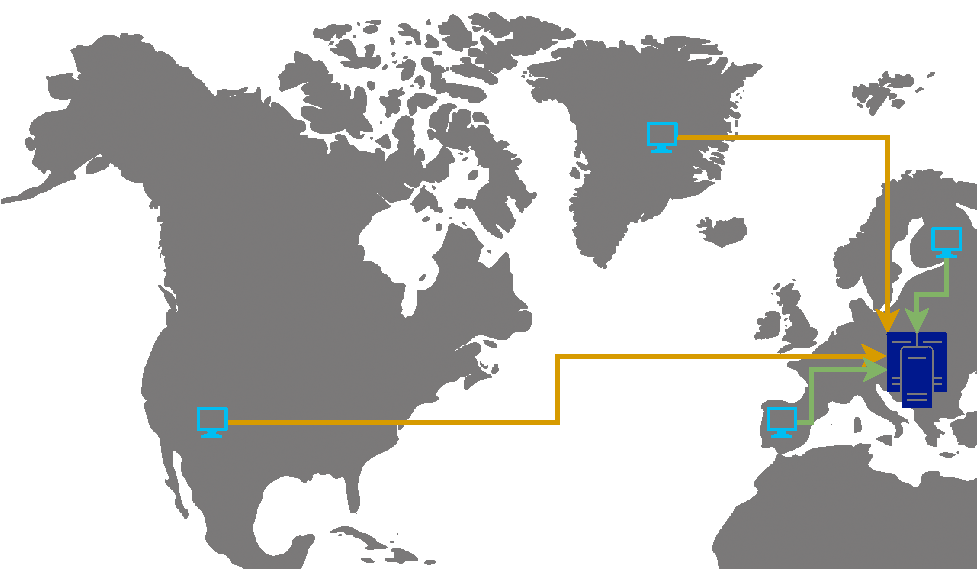
\includegraphics[width=1.0\textwidth]{images/problem-prevelike-latence.pdf}
\end{center}
\caption{Problem prevelike latence.}
\label{problem-prevelike-latence}
\end{figure}
\subsection{Višja razpoložljivost}
Vsakih nekaj let se zgodi, da je z interneta izpade kakšen večji podatkovni center. 
To se lahko zgodi iz več razlogov kot na primer večje napake na sistemu ali hujše vremenske razmere.
Če gre v takšnem primeru za večjega oblačnega ponudnika se to pozna tako, da je nezanemarljiv del interneta nedosegljiv.
Izpadi posameznih gruč pa se toliko pogosteje dogajajo, če gre za manjše ponudnike ali pa so naši strežniki v bolj nestabilnih okoljih. 
V splošnem se problem reši tako, da naše gruče namestimo v več podatkovnih centrov.
\subsection{Izolacija aplikacije}
Ko govorimo o izolaciji aplikacije se nanašamo na varnost pri vdoru, ali pa na večjo razpoložljivost.
Glede izolacije spletnih aplikacij smo z uporabo Kubernetesa naredili že kar nekaj korakov k dobri rešitvi problema.
Na primer vsaka aplikacija lahko teče v svojem kontejnerju, lahko pa jo celo izoliramo samo na določena vozlišča.
A vseeno se v Kubernetesu dogajajo problemi zaradi katerih postane cela gruča nedosegljiva.
Kaj takšnega se pogosto zgodi med posodabljanjem cele gruče.
Z varnostnega vidika pa mislimo na dejstvo, da če nekomu uspe serija napadov in se uspešno polasti enega samega vozlišča, si lahko začne lastiti celo gručo.
Ker ima administratorske pravice na vozlišču, ima posledično tudi popolno kontrolo nad vsemi drugimi aplikacijami, ki tečejo na tem vozlišču.
Aplikacije lahko pripadajo istemu uporabniku ali pa celo drugim uporabnikom.
Če imamo vsako od naših aplikacij v svoji gruči pa se temu lahko izognemo.
\subsection{Drag prenos podatkov}
Če se spustimo iz jedra računalniškega oblaka na njegov rob pa tam srečamo veliko zanimivih problemov. 
Na robu oblaka smo takrat, ko govorimo o delu naše aplikacije, ki se izvaja stran od centralnih aplikacij, ki so vedno doseljive.
Takšen primer so na primer mikro podatkovni centri in gruče na majhnih računalnikih kot na primer Raspberry PI.
Če naša aplikacija uporablja takšne gruče je potrebno tudi njihovo sinhrono delovanje.
Takšne majhne gruče so poleg že znanega problema prevelike razdalje pogosto obsojene, da s centralnimi strežniki komunicirajo minimalno, saj zelo pogosto za prenos podatkov uporabljajo draga mobilna omrežja.
\subsection{Razdeljevanje dela po različnih lokacijah}
Na robu oblaka pa se pogosto srečamo ne samo z omejenim komuniciranjem s centralnim strežnikom ampak tudi zmanjšano razpoložljivostjo in zmogljivostjo naprav.
Torej če ima ena gruča manj dela kot drugi lahko delež tega prenese na druge gruče.
\chapter{Problem povezovanja gruč}
Računalniška gruča je skupina računalnikov, ki zaradi večje zanesljivosti in zmogljivosti skupaj opravlja določene storitve.
Zaradi praktičnosti pa te storitve pogosto napišemo tako, da vsako storitev sestavlja več programov, ki tečejo v kontejnerjih.

Problem povezovanja več računalniških gruč je v svetu prisoten že kar nekaj časa.
Ko postavimo gručo, želimo da več računalnikov deluje kot celota, a z veliko večjo zanesljivostjo, stabilnostjo in zmogljivostjo.
Obstajajo primeri, ko bi radi med seboj povezali računalnike, a jih zaradi razdalje ali druačnih ovir ne moremo povezati v eno tesno povezano gručo.
V takšnih primerih pa pogosto lahko vsaj računalnike na isti lokaciji povežemo v gručo.
Te gruče pa potem na različne načine povežemo šibkeje.

Ko govorimo o tesni povezanosti znotraj gruče večinoma pričakujemo, da vsako vozlišče vidi vsako drugo, da vsak kontejner lahko komunicira z vsakim kontejnerjem, da so vozlišča v istem omrežju in da uporabljamo hitro interno omrežje podatkovnega centra. 
Pričakujemo, da sistem, ki ga uporabljamo za gručenje omogoča razporejanje zaželenih storitev in kontejnerjev med vozlišči in v primeru izpada vozlišča to vozlišče odstrani iz sistema in storitve s tega vozlišča prerazporedi na preostala vozlišča.

Ko pa govorimo o šibki povezanosti med različnimi gručami pa zaradi omejitev redko pričakujemo komunikacijo vsakega vozlišča z vsakim.
Zelo pogosto je povezava med vozlišči počasna, nezanesljiva in draga.
Po navadi je vsaka gruča v svojem omrežju in je to omrežje direktno nedosegljivo ostalim gručam.
Pričakujemo, da vsaka gruča skrbi za svoja vozlišča, ohranja svoje storitve in kontejnerje v delovanju.
Od sistema za povezovanje gruč pa si želimo, da nam omogoča centralni nadzor nad storitvami v gručah, prerazporejanje teh storitev med gručami, dinamično odkrivanje drugih gruč in njihovih storitev, izločanje nedosegljivih gruč, povezljivost med vsemi vozlišči in kontejnerji, četudi so vozlišča v različnih omrežjih.

\begin{figure}[h]
\begin{center}
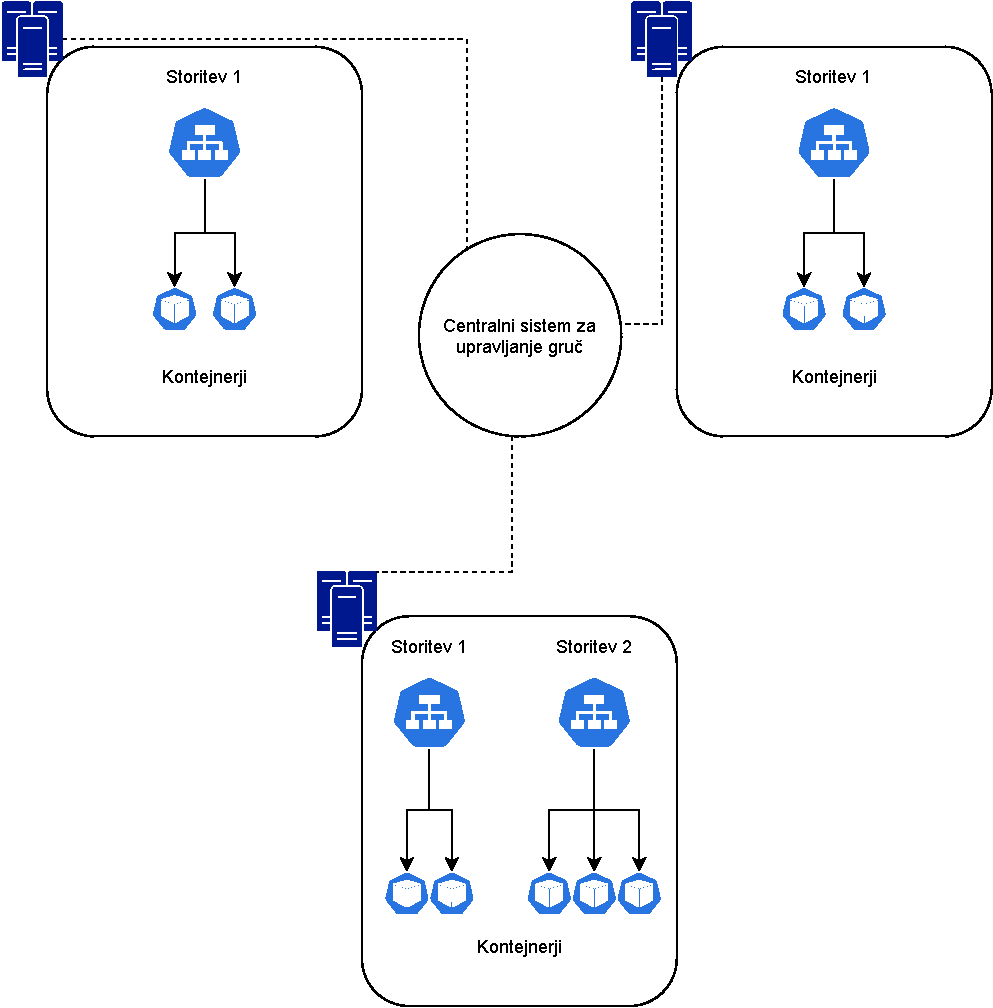
\includegraphics[width=1.0\textwidth]{images/primer-povezanih-gruc.pdf}
\end{center}
\caption{Primer povezanih več gruč.}
\label{problem-povezanih-gruc}
\end{figure}

\chapter{Kubernetes}
\label{Kubernetes}
Kubernetes definira javno dostopen REST API in trenutno obstaja že več kot 70 distribucij~\cite{cncf}.
Ko se bomo v tem dokumentu sklicevali na Kubernetes bomo imeli v mislih njegovo distribucijo.
\section{Zgodovina}
Leta 2014 je Google objavil in odprl kodo projekta Kubernetes~\cite{what-is-Kubernetes}.
Gre za program, ki je bil ustvarjen z namenom, da poenostavi upravljanje kontejnerjev in večjih računalniških gruč v produkcijskih okoljih.
A to vseeno niso pravi začetki Kubernetesa.
Začelo se je leta 2003, ko je Google začel z razvojem sistema za upravljanje njihovih internih gruč Borg.
Kasneje leta 2013 je Google predstavil sistem Omega.
Leta 2014 pa je Google objavil odprtokodni projekt Kubernetes. 
Projekt je bil zasnovan na podlagi dobrih praks upravljanja s kontejnerji, ki so se jih pri Googlu naučili skozi leta.
Kasneje je upravljanje nad projektom prevzela organizacija Cloud Native Computing Fundation.
\section{Osnovni pojmi}
Kubernetes API nam omogoča, da v Kubernetes shranjujemo najrazličnejše tipe objektov.
Takšne, ki so del standardnega kubernetesovega API-ja ali pa smo jih definirali sami (CRD).
Najpogostejši tipi objektov, ki se pojavijo v Kubernetesu so pod, service, deployment, statefulset in objekti za delo z diski.
\begin{figure}[h]
\begin{center}
\includegraphics[width=1.0\textwidth]{images/Kubernetes-simple-schema.pdf}
\end{center}
\caption{Primer delovanja Kubernetes objektov.}
\label{problem-povezanih-clustrov}
\end{figure}
\subsection{Pod~\cite{pod}}
Objekt pod običajno predstavlja nek primerek mikrostoritve.
Gre za najmanjšo enoto v Kubernetesu, ki lahko teče v gruči.
Sestavljen je iz enega ali več kontejnerjev, ki si delijo diske in omrežni vmesnik.
To pomeni, da imajo skupen IP in se obnašajo podobno kot izolirani procesi na istem računalniku.
\subsection{Service~\cite{service}}
Objekt service večinoma označuje vse pode ene mikrostoritve.
Kubernetes iz objekta v internem DNS ustvari domeno za mikrostoritev in dinamično razvršča promet med našimi podi.
Service objekte uporabljamo tako, da namesto pošiljanja zahtevkov direktno na IP naslov Poda, delamo klice na ustvarjeno domensko ime storitve na primer \spverb|curl ime-storitve|.
Takšen zahtevek potem dobi en izmed označenih podov v objektu service.
\subsection{Deployment~\cite{deployment}}
Deployment je objekt, ki mu podamo število željenih objektov pod in predlogo za njihovo izdelavo.
Potem pa interne storitve Kubernetesa zagotavljajo, da bo obstajalo toliko takšnih objektov tipa pod kot smo navedli v deploymentu.
Takšno stanje se poizkuša ohranjati tudi ob raznih težavah in izpadih vozlišč.
\subsection{StatefulSet~\cite{statefulset}}
Objekt zelo podoben deploymentu, le da statefulset vsaki replikaciji poda dodeli unikatno številko. 
Pod, ki se ustvari s to številko ohranja diske, mrežni vmesnik, IP naslov in domensko ime.
Pomembna razlika med objektoma deployment in statefulset pa je tudi v polju \spverb|volumeClaimTemplate|.
Statefulset omogoča vsakemu podu, da si ustvari in uporablja svoj disk.
Statefulset se najpogosteje uporablja za podatkovne baze in podobne storitve, ki morajo ohranjati stanja.
\chapter{Povezovanje Kubernetes gruč}
Ko postavimo več različnih gruč imamo vedno možnost, da upravljamo vsakega posebej~\cite{difference-multi-cluster}.
A takšen pristop zelo kmalu odpove, če imamo takšnih gruč res veliko.
Ko govorimo o sistemu, ki ga uporabljamo za upravljanje več gruč, najpogosteje pričakujemo možnost prenašanja objektov med gručami.
Tako lahko objekt definiramo samo enkrat in bo naš sistem ta objekt ustvaril v izbranih gručah.
Odvisno od naših potreb pa nam lahko prav pride tudi  dinamično odkrivanje storitev z enako definicijo v različnih gručah, komunikacijo med storitvami v različnih gručah, dinamično odkrivanje podov med gručami in komunikacijo med podi v različnih gručah.
Te funkcionalnosti znotraj ene gruče nudi že Kubernetes sam.
Je pa seveda odvisno od našega primera, katere funkcionalnosti želimo uporabiti in kako kompleksno postavitev potrebujemo.
V nadaljevanju si bomo ogledali različne sisteme za povezovanje Kubernetes gruč, njihove glavne prednosti in značilnosti.
  \section{ArgoCD in drugi GitOps}
\subsection{Sinhronizacija objektov z uporabo GitOps sistemov}
GitOps pristop pri postavljanju strukture aplikacij v Kubernetes gručah se je izkazal za dober pristop za upravljanje gruč.
Osnovna ideja GitOpsa je to, da imamo našo strukturo aplikacij v Kubernetes gruči napisano v repozitoriju Git in potem je kontroler GitOps tisti, ki iz teh definicij postavi strukturo gruče.
Če uporabljamo kakšnega od sistemov GitOps lahko potem iz enakega repozitorija postavimo več gruč.
V osnovi takšen pristop avtomatsko pomeni, da bomo imeli na voljo samo sinhronizacijo infrastrukture in nam takšen pristop ne omogoča naprednih funkcionalnosti kot so komunikacija med podi v različnih gručah ali pa odkrivanje storitev ali podov.
V nadaljevanju si bomo izbrali sistem ArgoCD in si pogledali kako bi si postavili zgoraj opisano infrastrukturo.
\subsection{Sinhronizacija objektov z ArgoCD}
ArgoCD podpira več različnih formatov konfiguracije gruče~\cite{argocd-docs}.
Najpreprostejše je, če uporabimo YAML format datoteke z definicijami objektov, ki jih želimo namestiti v vsako gručo.
Za deployanje te konfiguracije na več kot eno gručo imamo na voljo dva pristopa.
Prvi način je, da v vsako gručo namestimo ArgoCD in uporabimo enak repozitorij Git v vseh.
Drugi način, ki pa ga ponuja ArgoCD pa je, da lahko konfiguracijo pošljemo tudi v oddaljene gruče~\cite{declarative-setup}. To pomeni, da moramo imeti samo v eni gruči nameščen ArgoCD kontroler.

Pogosto pa ne želimo, da imajo vse gruče popolnoma enako infrastrukturo in želimo vsaj malo prilagoditi konfiguracijo posameznege gruče.
V tem primeru bi uporabili format zapisa konfiguracije, ki podpira predloge.
ArgoCD nam ponuja možnost, da ročno določimo spremenljivke predlogam.
Tako lahko uporabimo na primer predloge HELM in ArgoCD nam bo omogočil, da vsaki gruči izberemo svojo datoteko s spremenljivkami.
Glede na preprostost delovanja takšnega sistema se moramo zavedati, da od njega ne moremo pričakovati nikakršnih naprednih funkcionalnosti kot sta dinamično odkrivanje storitev ali komunikacija podov med gručami.
Takšen sistem nam omogoča samo sinhronizacijo infrastrukture.

\begin{figure}[h]
\begin{center}
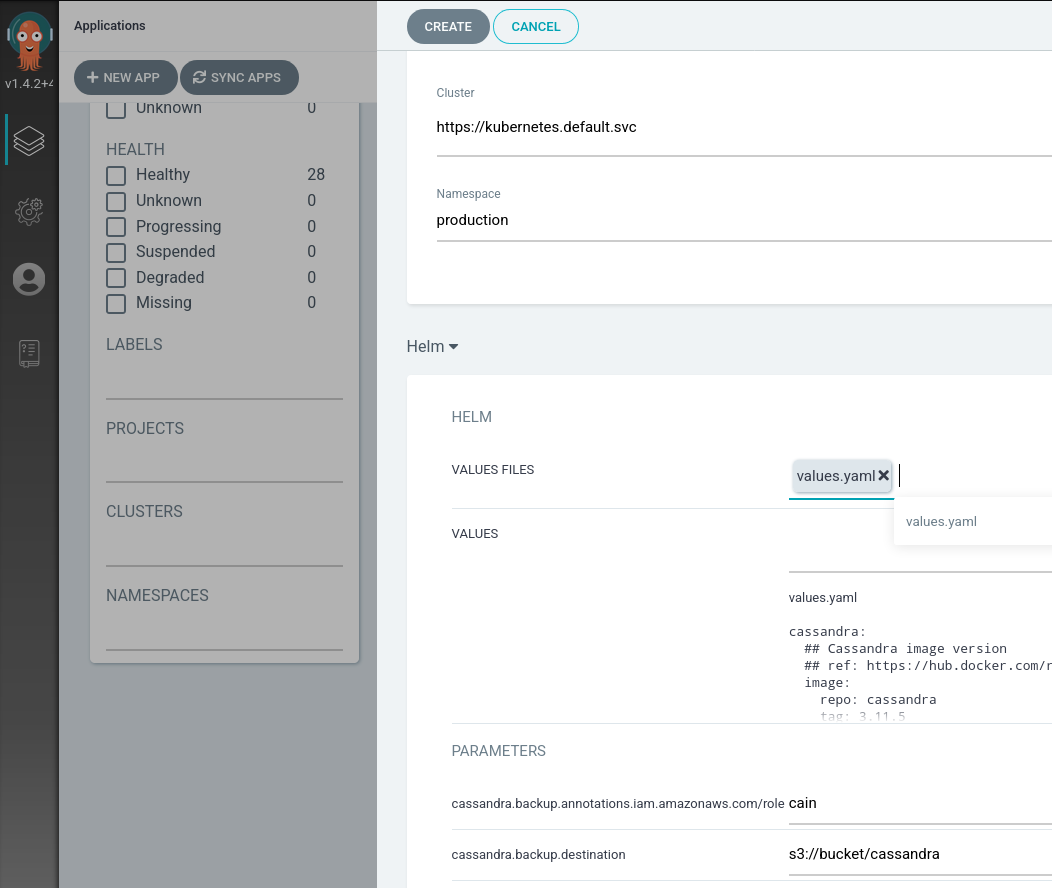
\includegraphics[width=1.0\textwidth]{images/primer-uporabe-helm-predloge-argo-cd.png}
\end{center}
\caption{Primer uporabe helm predloge v ArgoCD.}
\label{primer-uporabe-helm-predloge-argo-cd}
\end{figure}


\section{KubeFed}
9. 1. 2018 je bil po ukinjenem projektu Kubernetes Federation V1 ustvarjen Kubernetes Federation V2 ali KubeFed~\cite{Kubernetes-federation-evolution}.
Oba projekta sta želela poenostaviti upravljanje več gruč in razporejanje Kubernetes objektov.
V projektu Federation V1 je bil ubran pristop, ki je skupino gruč ali federacijo uporabniku predstavil kar kot novo Kubernetes gručo~\cite{setup-cluster-federation-kubefed-v1}.
Uporabljal je svoj API in API kontroler, ki pa je bil združljiv s Kubernetesovim, kar pa je omogočalo tudi uporabo orodja kubectl~\cite{cluster-federation-in-Kubernetes-1.5}.
Objekti, ki jih je federacija podpirala so bili kompatibilni s standardnimi Kubernetes objekti~\cite{federated-cluster-kubefed-v1}.
Takšne objekte je potem Federation V1 ustvaril tudi v ostalih gručah.
Zanimiv pristop, ki pa zaradi mnogih pomanjkljivosti in pomankanja možnosti naprednejših konfiguracij ni uspel pridobiti statusa GA.
GA faza v Kubernetesu pomeni, da se uporabniki lahko zanašajo na projekt, ga uporabljajo in se bo vsaj do neke mere ohranjala združljivost za nazaj.
Pred dosegom te stopnje naj bi se projekt uporabljalo samo v testne namene.

Tako se je kasneje rodil projekt Federation V2~\cite{Kubernetes-federation-evolution}.
Glavna razlika s prvo verzijo z uporabniškega stališča je v tem, da za federacijo ne poizkuša imitirati Kubernetesovega API-ja, ampak uporablja obstoječi Kubernetesov API. 
Federation V2 samo predstavi nove objekte, ki pa so razširitev standardnih, kot na primer federateddeployment.
Federated objekte je treba najprej vklopiti z ukazom \spverb|kubefedctl| enable.
\begin{verbatim}
kubefedctl enable deployment
\end{verbatim}
Orodje kubefedctl si moramo namestiti na naš računalnik.
Takšen Federated objekt vsebuje tri glavne lastnosti: definicija predloge primarnega objekta, postavitev v gruče in prepis lastnosti originalnega objekta za posamezne gruče.
  Takšen pristop je zelo široko zastavljen in omogoča tudi federacijo CRD objektov.
\begin{verbatim}
apiVersion: types.kubefed.io/v1beta1
kind: FederatedDeployment
spec:
  placement:
    clusterSelector:
      # izbira gruč
      matchLabels: {}
      ... 
  template:
    # specifikacije deployment objekta
    spec:
    ... 
  overrides:
    # prepis konfiguracije za posamezne gruče
    - clusterName: gruca-1
      clusterOverrides:
          # nastavi polje replicas na vrednost 5
        - path: "/spec/replicas"
          value: 3
  ... 
\end{verbatim}
Federation V2 podpira poleg sinhronizacije infrastrukture tudi odkrivanje storitev v drugih gručah prek DNS zapisov.
Omenja pa se možnost odstranitve te funkcionalnosti~\cite{remove-service-discovery}, ki je že sedaj privzeto izklopljena.
Preden pa uporabimo KubeFed pa se moramo zavedati, da je projekt v času pisanja diplomske naloge še vedno v razvojni fazi alfa in lahko mine še nekaj časa preden doseže status GA, če slučajno ne bo šel po stopinjah svojega predhodnika.
\section{Cilium}
Cilium je odprtokodni program, ki nam omogoča napredne varnostne in omrežne nastavitve v naši gruči~\cite{cilium-intro}.
Program na tretji in četrti omrežni plasti zagotavlja osnovne principe varnosti in zaščite, kot na primer zapiranje portov in omejevanje komunikacije.
Poleg tega pa Cilium zagotavlja tudi naprednejšo varnost na sedmi omrežni plasti, saj nam omogoča omejevanje in filtriranje HTTP zahtevkov in podobne varnostne funkcionalnosti na popularnih protokolih aplikacijskega nivoja~\cite{cilium-intro}.

Ker Cilium implementira precejšni del mreženja in povezovanja v Kubernetesu, pa nam s tem lahko ponudi tudi nekaj zelo naprednih možnosti, ko med seboj povezujem več različnih Kubernetes gruč.
Tako nam kot ključno prednost Cilium omogoča tudi komunikacijo med podi v različnih gručah~\cite{cilium-cluster-mesh} in uporabo globalnih objektov service, ki so sposobni delati razporejanje prometa med različnimi gručami.
Takšne objekte definiramo z anotacijo io.cilium/global-service~\cite{setup-cilium-cluster-mesh}.
Omogoča nam tudi omejevanje povezovanja med gručami z njihovim objektom CiliumNetworkPolicy~\cite{setup-cilium-cluster-mesh}.
Ko postavljamo mrežo gruč, pa se moramo še vedno zavedati, da Cilium ne rešuje problema, če so naše gruče skrite v različnih zasbenih omrežjih.
Ključno pri uporabi Ciliuma za povezovanje gruč je, da so vsa naša vozlišča dosegljiva med seboj.
A četudi so naše gruče v med seboj nedosegljivih zasebnih omrežjih, pa je problem z lahkoto rešljiv z uporabo sistema VPN, ki nam omogoča, da vsa vozlišča povežemo v eno virtualno omrežje~\cite{setup-cilium-cluster-mesh}.

Kljub naprednim funkcijam, ki nam jih Cilium ponuja, pa se moramo zavedati, da se Cilim ukvarja samo s povezovanjem gruč na omrežnem nivoju.
Ne omogoča enotnega upravljanja in sinhroniziranja objektov med gručami zato moramo objekte sinhronizirati sami.
Ampak zaradi dovolj široke zasnove Kubernetesovega vmesnika so rešitve med seboj kompatibilne.
Torej lahko uporabimo napredno mreženje Ciliuma in objekte sinhroniziramo s KubeFed in GitOps pristopom.
\chapter{Priprava sistema gruč za testiranje}
\section{Raspberry PI 4}
Za namene testiranja različnih načinov povezovanja Kubernetes gruč moramo najprej postaviti nekaj gruč.
Zaradi preprostosti in nizke cene, predvsem pa ker se koncepti zaradi tega ne spremenijo, bomo za naša Kubernetes vozlišča uporabili Raspberry PI 4.
Na višjem nivoju pa gre še vedno za Kubernetes gručo in je delo zelo podobno, če uporabimo nekaj 1000 vozlišč v gruči v oblaku ali pa lokalno gručo z enim vozliščem.
Raspberry PI je zelo majhen in manj zmogljiv računalnik na eni sami plošči.
Ključni prednosti takšnih računalnikov pa sta prav velikost in cena.
Na vsak Raspberry PI se bo namestila Kubernetes gruča z enim samim vozliščem.
Fizična postavitev gruč je prikazana na sliki \ref{rpi-gruce}.
Takšna postavitev pa je lahko tudi primer gruče na robu oblaka, kar je bolj podrobno opisano v poglavju \ref{edge-clusters}.
\begin{figure}[h]
\begin{center}
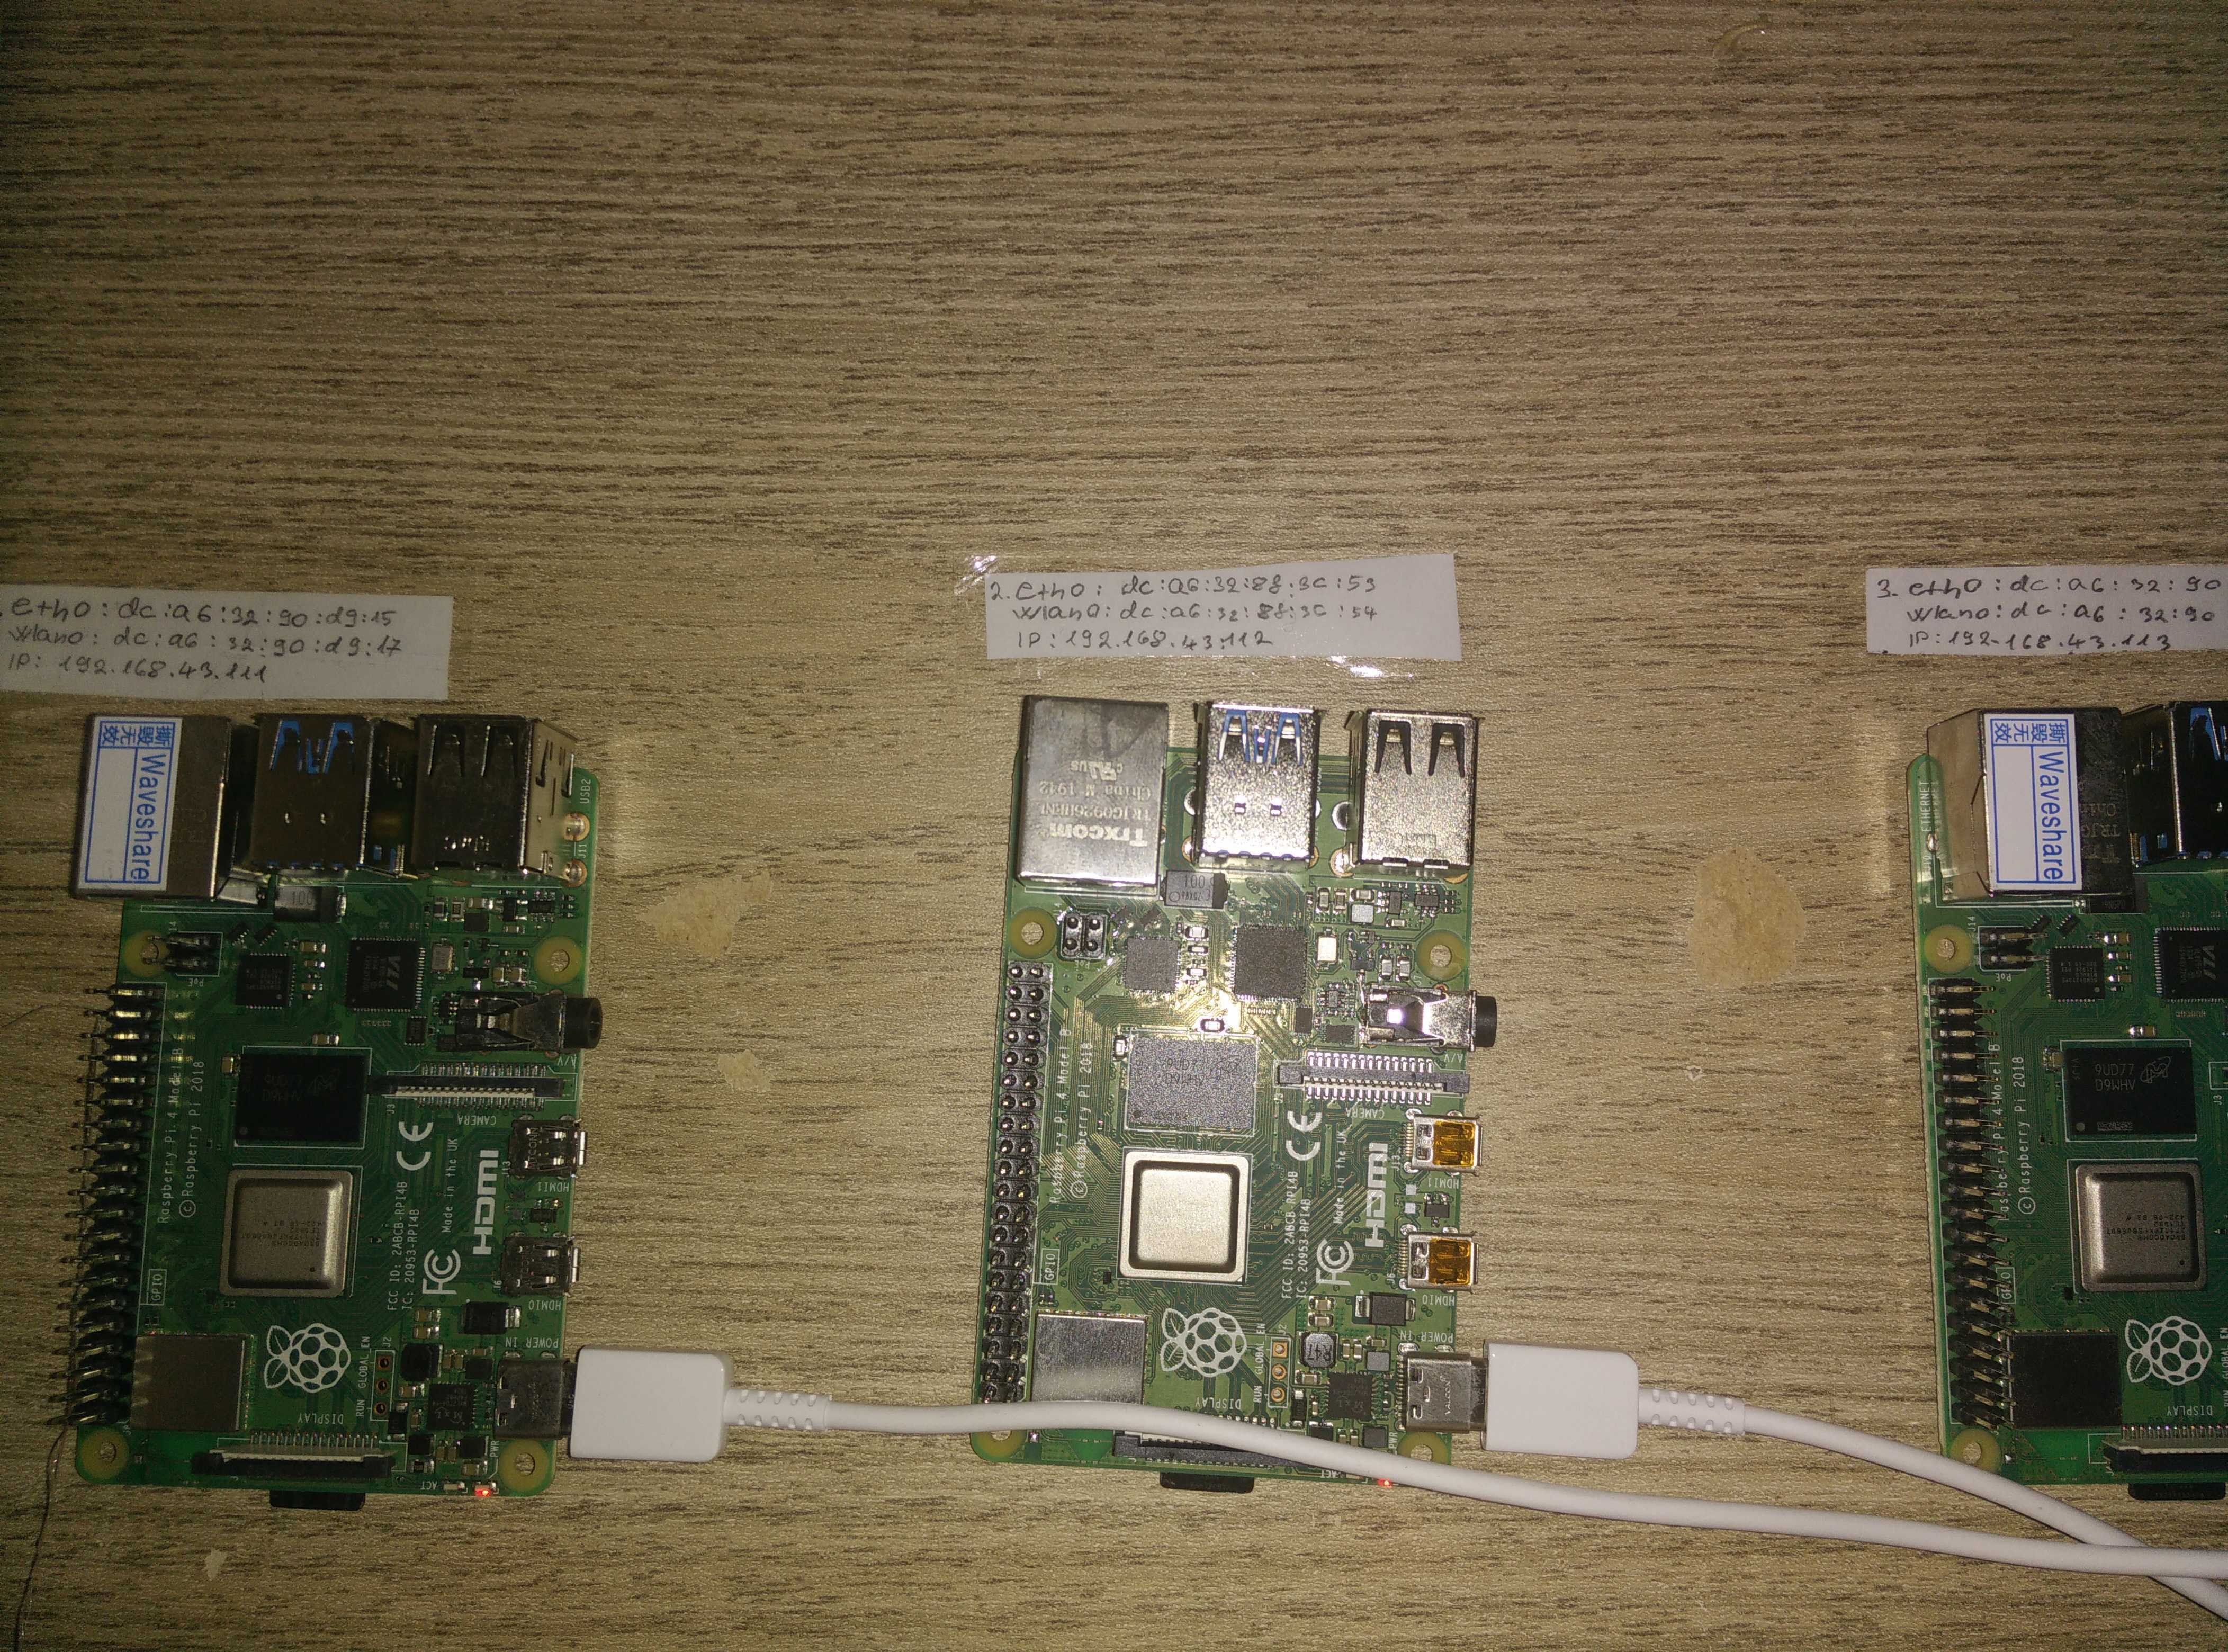
\includegraphics[width=1.0\textwidth]{images/postavitev-raspberry.jpg}
\end{center}
\caption{Postavitev Raspberry PI gruč.}
\label{rpi-gruce}
\end{figure}
\section{K3S in K3OS}
Obstaja več implementacij Kubernetesa in mi bomo uporabili z viri varčno odprtokodno implementacijo K3S od podjetja Rancher~\cite{k3s-info}.
Hkrati so v podjetju Rancher pripravili distribucijo operacijskega sistema Linux K3OS, ki jo lahko namestimo na katerikoli računalnik~\cite{k3os-git}. 
Majhna težava se pojavi, ker še ni pripravljene uradne verzije operacijskega sistema za ploščice Raspberry PI.
A k sreči se je v ta namen začel odprtokodni projekt PiCl k3os image generator, ki nam iz slik operacijskih sistemov K3OS in Raspberry OS in konfiguracijskih datotek zgradi novo sliko operacijskega sistema za naš Raspberry PI ~\cite{k3os-rpi-image-generator}.
Konfiguracijske datoteke, ki jih moramo priložiti so standardne YAML datoteke, ki jih podpira K3OS.
Vanje zapišemo nastavitve kot so SSH javni ključi za dostop, podatki od WiFi omrežja na katerega se povezujemo, geslo, žeton za povezavo s Kubernetes gručo in način v katerem želimo zagnati K3S na sistemu~\cite{k3os-git}.
\begin{figure}[h]
  \begin{verbatim}
ssh_authorized_keys:
- ssh-rsa ...
hostname: gruca-1
k3os:
  ntp_servers:
  - ...
  password: ...
  token: ...
  dns_nameservers:
  - ... 
  wifi:
  - name: ...
    passphrase: ...
  k3s_args:
  - server
\end{verbatim}
\end{figure}
  V našem primeru smo vse K3S programe zagnali v strežniškem načinu in nobenega v načinu delovnega vozlišča, saj želimo, da vsak Raspberry PI predstavlja svojo gručo.
\section{Demonstracijska spletna aplikacija}
Za potrebe testiranja je bilo potrebno naredili novo testno mikrostoritev.
Ker se v tem diplomskem delu želimo osredotočiti na resnične probleme v industriji, mora ta aplikacija omogočati tudi shranjevanje podatkov v podatkovno bazo.

Koda, ki je javno objavljena v Git repozitoriju~\cite{git-stateful-rest-sample}, je napisana v programskem jeziku Go.
Iz kode je bil generiran kontejner, ki je objavljen v javnem Docker repozitoriju~\cite{docker-stateful-rest-sample}.
Ob tem velja opozoriti, da Raspberry PI uporablja ARM arhitekturo procesorja, kar je zahtevalo posebno pozornost.

Aplikacija deluje preprosto.
Na mrežnih vratih podanih s spremenljivko okolja izpostavi vmesnik REST z dvema preprostima HTTP klicema.
GET klic na pot \spverb|/users| nam bo vrnil vse uporabnike, ki so zapisani v tabeli v bazi, s klicem POST na isto pot pa poskrbimo, da se podatki uporabnika iz našega zahtevka shranijo v tabelo v bazo.
\begin{verbatim}
# ukaz za dodajanje uporabnika
curl -X POST localhost/users \
  --data '{"name": "John", "lastname": "Doe"}'
# ukaz za prikaz vseh uporabnikov
curl localhost/users
\end{verbatim}

Za shranjevanje podatkov bomo uporabili 2 različni SQL bazi podatkov.
Postgres, ki je preprosta za lokalni razvoj, a ne omogoča napredne sinhronizacije podatkov med strežniki in CrateDB, ki je bil zasnovan kot SQL baza na več vozliščih in nam omogoča napredne sinhronizacije tudi med različnimi strežniki in gručami.
K sreči pa CrateDB implementira PostgreSQL vmesnik in nam kode za prehod med bazami ni potrebno spreminjati.
\section{Namestitev KubeFed}
Kot ena izmed ključnih komponent složnega delovanja več gruč je njihovo upravljanje.
V te namene bomo uporabili program KubeFed, ki ga moramo namestiti na eno izmed gruč, ki jih želimo povezati skupaj.
Ker je izdelek še v razvoju in še ni prišel iz alfa faze, nimajo objavljene verzije za procesorje ARM.
Zato je bilo iz kode KubeFed potrebno zgraditi novo sliko kontejnerja, ki je javno objavljena~\cite{docker-kubefed}.
Potem pa smo uporabili originalno Helm predlogo, kjer smo samo zamenjali originalno sliko kontejnerja z našo.
Za delo s KubeKed pa moramo na svoj računalnik namestiti orodje kubefedcli.
Z uporabo ukaza \spverb|kubefedctl join| povežemo vse tri gruče v kubefed sistem.
\begin{verbatim}
kubefedctl join gruca-1
kubefedctl join gruca-2
kubefedctl join gruca-3
\end{verbatim}
S tem smo uspešno povezali več Kubernetes gruč v sistem KubeFed.
Seznam vseh povezanih gruč pa lahko preverimo tako, da izpišemo seznam objektov tipa kubefedclusters. 
V našem primeru imamo povezane tri gruče, kar se vidi iz sledečega izpisa.
\begin{verbatim}
kubectl get kubefedclusters

NAME        AGE   READY
gruca-1     1d    True
gruca-2     1d    True
gruca-3     1d    True
\end{verbatim}
Sedaj lahko z uporabo ukazov \spverb|kubefedctl enable| in \spverb|kubefedctl federate| naše objekte dodajamo v vse gruče hkrati.
Več o tem je napisano v poglavjih, kjer ukaze tudi uporabljamo.

\chapter{Povezovanje med podatkovnimi centri}
\label{povezovanje-med-centri}
\section{Problem velike latence}
V industriji je zelo malo primerov spletnih aplikacij, ki jim ni potrebno hraniti stanja. 
Ko neko podjetje, lastnik aplikacije poseže po globalnem trgu zelo hitro ugotovi, da stranke, ki niso blizu podatkovnega centra precej dlje čakajo pred ekrani, da se naloži njihova spletna aplikacija in njihovi podatki.
Takšen problem se v splošnem rešuje tako, da našo aplikacijo postavimo še na dodaten strežnik bližje uporabniku. 
Rešitev se sliši preprosta, a vseeno se tu srečamo z zelo zahtevnimi problemi v računalništvo.
Najbolj očiten primer je sinhronizacija podatkov.
V našem primeru bomo uporabili podatkovno bazo CrateDB~\cite{cratedb}, novejšo alternativo standardnim SQL podatkovnim bazam.
CrateDB ima v primerjavi s tradicionalnimi podatkovnimi bazami boljšo podporo za sinhronizacijo podatkov med vozlišči.
Poleg vsega pa nam za uporabo podatkovne baze CrateDB ni potrebno konceptualno spreminjati naše aplikacije, saj podpira vmesnik od podatkovne baze PostgreSQL.
\section{Povečanje razpoložljivosti aplikacije}
Če je čim višja razpoložljivost za našo aplikacijo kritičnega pomena in smo že poskrbeli za visoko razpoložljivost (HA) aplikacije v naši gruči, še vedno lahko pride do situacije, ko iz omrežja izpade cel podatkovni center.
Spomnimo se, da Kubernetes najbolj učinkovito deluje, če naša vozlišča uporabljajo hitro interno omrežje podatkovnega centra.
V primeru naravnih nesreč ali hujših vremenskih pogojev pomeni, da je nedosegljiv cel podatkovni center in s tem gruča v njem.
Če uporabljamo oblak, pa gremo lahko še korak dlje z zagotavljanjem razpoložljivosti.
Če nam ni dovolj niti to, da uporabimo različne razpoložljivostne cone in podatkovne centre oblačnih ponudnikov, lahko postavimo naše gruče pri več različnih ponudnikih.
Tu Kubernetes pride zelo do izraza, saj kljub nekaj neenakostim skozi implementacije ohranja enak vmesnik in je zato takšna postavitev precej lažja, kot bi bila brez uporabe Kubernetesa.
\section{Povezovanje med podatkovnimi centri}
Rešitev za oba problema je identična.
Postaviti moramo gruče v več različnih podatkovnih centrih in jih nastaviti, da bodo delovali usklajeno.
Odvisno od problema bodo te podatkovni centri morda bližje uporabniku, morda v lasti različnih oblačnih ponudnikov ali pa oboje.
Ampak princip ostaja enak.
\section{Razporeditev uporabnikov po gručah}
Ko imamo na vsaki gruči javno izpostavljen Kubernetesov service objekt in postavljene primerne ingress objekte, moramo še vedno uporabnike preusmeriti na njim najbližjo gručo.
Uporabnike lahko mi usmerimo avtomatsko z DNS zapisi, ki omogočajo usmerjanje na podlagi geolokacije.
Lahko uporabimo in namestimo zunanji DNS skozi Kubernetes ali pa to opravimo kar mimo Kubernetesa.
V naših lokalnih testnih gručah bomo ta korak preskočili in jih ne bomo usmerjali preko javnih DNS strežnikov, saj v lokalnem okolju to ni smiselno.
\begin{figure}[h]
\begin{center}
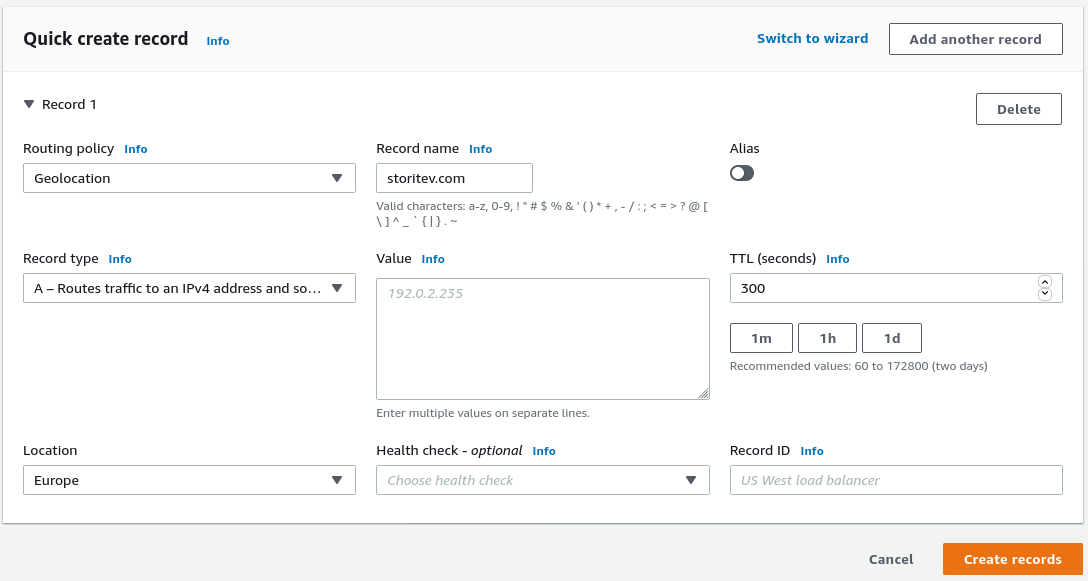
\includegraphics[width=1.0\textwidth]{images/geolokacijski-dns.png}
\end{center}
\caption{Ustvarjanje geolokacijskega DNS zapisa v storitvi ROUTE53.}
\label{primer-ustvarjanje-geolokacijskega-zapisa}
\end{figure}

Naslednja možnost pa je rešitev, ki se jo zelo pogosto poslužujejo internetne računalniške igre, da so naši strežniki popolnoma ločeni in se vsak uporabnik sam odloči na kateri gruči ali strežniku želi igrati.
V takšnih primerih se lahko tudi izognemo problemu sinhronizacije podatkov med strežniki, kar zelo poenostavi upravljanje naših gruč.
\section{Definicija infrastrukture za naš primer}
V našem primeru spletne aplikacije bomo imeli v vsaki gruči eno postavitev aplikacije \sn{Stateful rest sample} z deployment objektom. 
Da pa aplikacijo izpostavimo izven gruče, pa bomo uporabili objekt service.
Aplikacija bo za shranjevanje uporabljala podatkovno bazo CrateDB, ki bo postavljena z objektom statefulset, diskom na lokalni SD kartici, in dvema objektoma service.
Prvi objekt service je zunanji in se bo uporabljal za dostop do baze, drugi pa je notranji in ga bomo uporabljali za prepoznavo ostalih primerkov CrateDB v gruči.
\begin{figure}[h]
\begin{center}
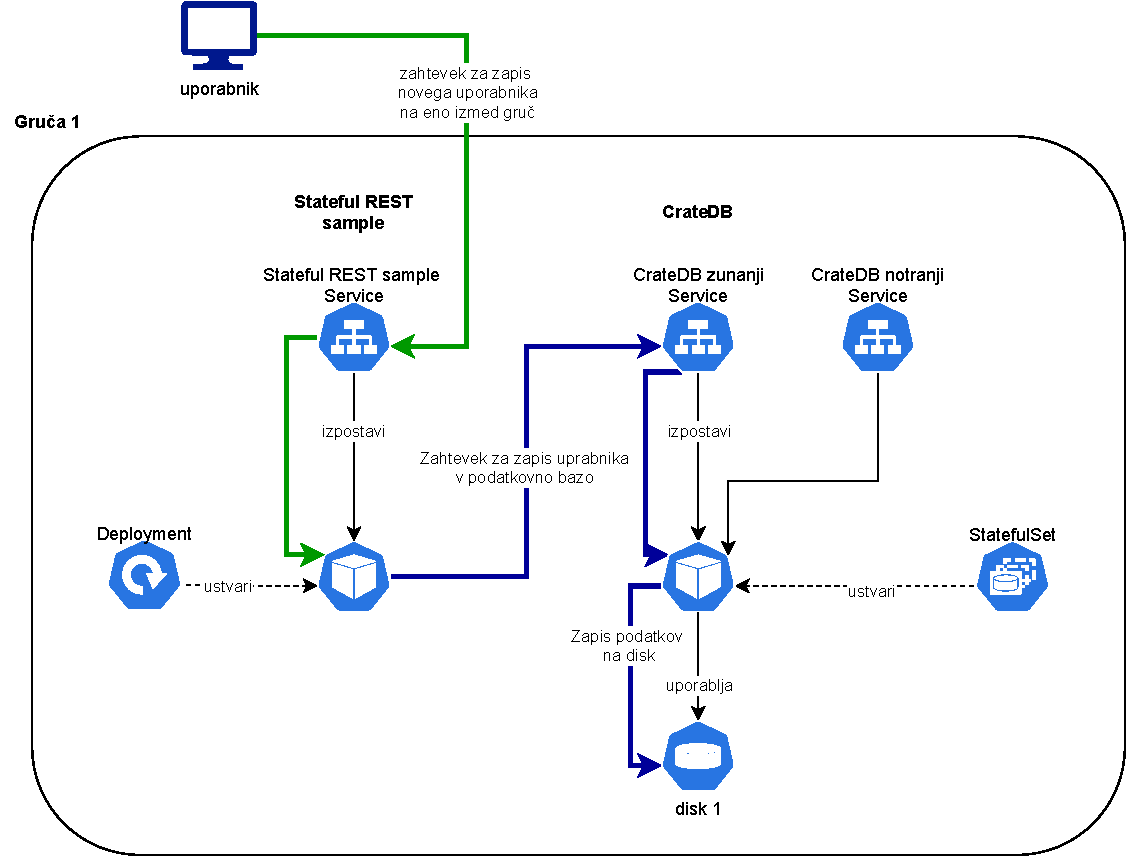
\includegraphics[width=1.0\textwidth]{images/infrastructure-example.pdf}
\end{center}
\caption{Infrastruktura vsake gruče v primeru demonstracijske aplikacije}
\label{primer-uporabe-helm-predloge-argo-cd}
\end{figure}
Vsa konfiguracija je javno objavljena na Git repozitoriju\cite{git-diploma}. Postavimo jo z ukazom \spverb|kubectl apply -f diploma-demo-1|
Takoj preverimo, če aplikacija deluje in če lahko podatke zapisujemo v bazo, tako da prek demo aplikacije poizkusimo dodati uporabnika in izpisati vse uporabnike.
To naredimo z naslednjima \spverb|curl| ukazoma.
\begin{verbatim}
curl -X POST gruca-1/users \
    --data '{"name": "John", "lastname": "Doe"}'
curl gruca-1/users
\end{verbatim}
\section{Implementacija s KubeFed}
Najprej se moramo odločiti za katere tipe objektov bomo vklopili federacijo oziroma za katere bomo želeli univerzalno upravljanje.
V našem primeru gre za service, deployment in statefulset. Vklopimo jih z naslednjim ukazom, ki za nas ustvari nove federated tipe objektov na izbranih tipih.
\begin{verbatim}
kubefedctl enable <ime tipa>
\end{verbatim}
Ko smo si vklopili federacijo na vseh potrebnih tipih pa moramo še vklopiti avtomatsko upravljanje na specifičnih objektih.
V našem primeru želimo za to uporabiti ukaz \spverb|kubefedctl federate|.
\begin{verbatim}
kubefedctl federate deployment stateful-rest-sample
kubefedctl federate service stateful-rest-sample
kubefedctl federate statefulset crate
kubefedctl federate service crate-internal
kubefedctl federate service crate-external
\end{verbatim}
Izvršeni ukazi ustvarijo federated objekte, ki uporabijo postavitev v vse gruče in za predlogo kar podane objekte.
Tako je za nas rezultat izvršenih ukazov kreiranje federated objektov in posledično kopiranje objektov v vse naše povezane gruče.

Po preizkusu delovanje s \spverb|curl| ukazom opazimo, da podatki med gručami še vedno niso sinhronizirani.
Uporabniki, ki jih vnesemo v eno gručo se še ne sinhronizirajo v ozadju.
Na tej točki se ustavijo nekatere spletne aplikacije in prepustijo izbiro strežnika oziroma gruče kar uporabniku.
\section{Sinhronizacija podatkov}
Če želimo pred uporabnikom skriti, da uporabljamo več gruč, moramo poleg geolokacijskih DNS zapisov, urediti tudi avtomatsko sinhronizacijo podatkov.
Sicer v našem primeru res uporabljamo samo en primerek CrateDB baze na gručo, a vseeno smo na nivoju sinhronizacije znotraj gruče to stvar že uredili. 
Zopet se moramo spomniti, da so tudi gruče podatkovnih baz pogosto narejene tako, da najbolje delujejo, če so vozlišča v hitrem lokalnem omrežju.
Zaradi tega mnoge baze, ki podpirajo sinhronizacijo podatkov znotraj gruče, podpirajo tudi sinhronizacijo med različnimi podatkovnimi centri.
\subsection{Uporaba primerne podatkovne baze}
Najlažje je sinhronizirati podatke, če uporabimo podatkovno bazo, ki ima sinhronizacijo med različnimi gručami že podprto.
CrateDB podpira sinhronizacijo tudi preko razpoložljivostnih con.
Vseeno pa je mišljeno, da vsa vozlišča povežemo v enako podatkovno gručo.
To pomeni, da morajo vsa vozlišča imeti dostop do vseh.
Zelo elegantna rešitev bi bila uporaba sistema Cilium in uporaba globalnih storitev, saj nam Cilium že omogoča komunikacijo vsakega poda z vsakim, tudi če so ti v različnih gručah.
Druga možnost pa je, da izpostavimo vsak pod s svojim javnim IP naslovom in jih ročno povežemo v gručo.

Potem pa moramo nastaviti še nastavitve, ki jih baza podpira za zmanj\-šan\-je prometa in zagotavljanje željene razpoložljivosti med gručami~\cite{cratedb-zone}.
Podobne načine sinhronizacije podpira tudi na primer podatkovna baza Cassandra~\cite{cassandra-zone}.
\subsection{Podatke sinhroniziramo sami}
Sinhronizacija podatkovne baze je težak problem.
Če ne uporabimo primerne podatkovne baze ali pa želimo sinhronizirati samo določene stvari preko gruč bomo sinhronizacijo podatkov verjetno morali napisati sami.
To pomeni, da bomo ustvarili novo mikrostoritev, ki bi v ozadju kopirala ključne podatke med podatkovnimi centri.
Ker samo mi poznamo naš konkreten primer uporabe, je takšen pristop lahko najbolj učinkovit.

V našem primeru bomo s preprosto skripto kopirali uporabnike iz ene aplikacije v drugo kar z uporabo našega REST vmesnika.
To bomo storili v drugem Ubuntu kontejnerju z uporabo ukazov \spverb|curl| za izvajanje REST klicev in ukazom \spverb|jq|~\cite{jq} za razčlenjevanje podatkov.
Podatki se sinhronizirajo vsakih 10 sekund.
Primer še testiramo in dobimo spodnji izhod, kar potrdi, da so se podatki uspešno sinhronizirali.
\begin{verbatim}
curl -s -X POST gruca-1/users|jq \
  --data '{"name": "John", "lastname": "Doe"}'
curl -s gruca-2/users|jq
[{"Name":"John","Lastname":"Doe"}]
\end{verbatim}
\chapter{Upravljanje izoliranih aplikacij}
\section{Zmanjševanje posledic vdorov in izpadov}
  Računalniška stroka si je že nekaj časa nazaj priznala, da popolnega sistema ne more ustvariti: sistema, ki se ne more sesuti, sistema, ki bo ves čas razpoložljiv in sistema, v katerega ne bo mogoče vdreti.
To vsake toliko časa potrdijo tudi najbolje upravljani veliki sistemi kot so AWS, Google, Facebook z izpadi ali vdori na njihovih storitvah. 
Vseeno pa kljub vdorom in napakam, zaradi katerih postanejo naši sistemi nedosegljivi, vedno lahko poizkusimo zmanjšati posledice ob morebitnem vdoru ali napadu. 
\subsection{Izpadi aplikacije}
Kljub temu, da smo naše aplikacije namestili na različne gruče in je s tem aplikacija odporna na izpad ene gruče, pa lahko ob hujših nepravilnostih delovanja ene aplikacije in napaki pri nastavitvi gruč kaskadno izpadejo tudi vse gruče na katerih imamo aplikacijo nameščeno.
Takšen primer bi bil, če ena aplikacija ali mikrostoritev zavzame vse vire v gruči hkrati pa odpovejo ostale varovalke, ki jih ponuja že sam Kubernetes.
V takšnih primerih bo odpovedal cel naš sistem namesto samo del sistema.
Zato se lahko odločimo, da bomo nekatere bolj kritične aplikacije ali mikrostoritve postavili v gručo, kjer napake drugih aplikacij ne bodo vplivale na naše delovanje.
A vseeno se moramo zavedati, da je ta korak smiseln šele ko smo opravili že vse predhodne preventivne ukrepe, kot so razdelitev aplikacije na mikrostoritve, kontejnerijzacija, izolacija na posamezno Kubernetes vozlišče, pravilna nastavitev omejitev avtomatskega povečevanja in še mnoge druge.
\subsection{Vdori}
Podobno kot pri izpadih aplikacije je tudi pri preprečevanjih posledic vdorov.
Najprej moramo poskrbeti za primerno zaščito Kubernetes vozlišč, naše aplikacije, kriptiranje komunikacije med mikrostoritvami, uporabo nepriviligiranih in neadministratorskih kontejnerjev.
Če pa nam vsi zgoraj našteti in ostali priporočeni ukrepi niso dovolj ali pa se zavedamo, da imamo v gručah manj varne aplikacije in napadalec prek teh aplikacij ne sme dostopati do podatkov kritičnih aplikacij, potem pa je smiselno kritične aplikacije izolirati v svoje gruče.
\section{Implementacija s Kubefed}
\begin{figure}[h]
\begin{center}
  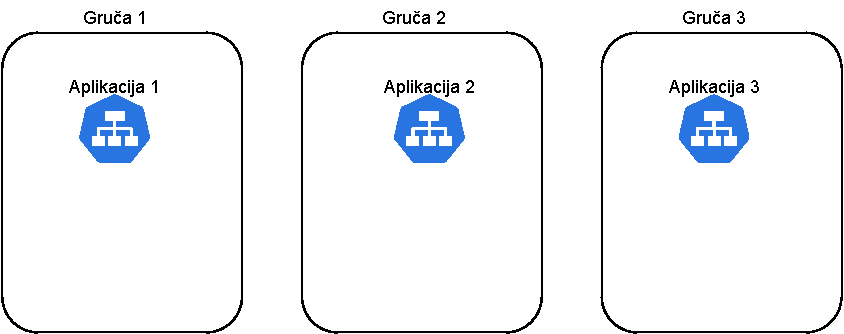
\includegraphics[width=1.0\textwidth]{images/primer-izolirane-aplikacije.pdf}
\end{center}
\caption{Primer izoliranih aplikacij.}
\label{problem-prevelike-latence}
\end{figure}
Ena izmed treh glavnih lastnost federiranih objektov je možnost izbire gruč na katerih se bo določen objekt ustvaril. 
S tega stališča je naš primer zelo preprost.
Samo določimo da se naša aplikacija izvaja na gruči 3 namesto na vseh.
Tokrat za federacijo ne moremo uporabiti ukaza \spverb|kubefedctl federate|, ampak moramo spisati konfiguracijo federiranih objektov sami.
Najprej bomo z ukazom \spverb|kubectl tag| označili našo izolirano gručo (ali več njih).
Potem pa bomo lastnosti \spverb|.clusterSelector.matchLabels| vsakega federiranega objekta, ki ga želimo izolirati, dodali označbe vseh izoliranih gruč.
V takšnih primerih se nam ni potrebno posebej ukvarjati s sinhronizacijo podatkov, saj smo ali vse podatke obdržali v isti gruči ali pa sinhroniziramo na enak način kot v poglavju \ref{povezovanje-med-centri}.
\chapter{Upravljanje gruč na robu oblaka}
\label{edge-clusters}
\section{Gruče na robu oblaka}
Razlogov zakaj gruče postavljamo na rob oblaka oziroma fizično bližje konč\-ne\-mu uporabniku je več.
Pogosto ne želimo na glavni strežnik pošiljati vseh podatkov, ampak želimo podatke obdelati že lokalno, da lahko po omrežju pošiljamo samo agregirane podatke.
Smiselnost takšne postavitve pride še posebej do izraza, če podatke prenašamo po dragem mobilnem omrežju.
A možnih postavitev in razlogov zanje pa je več.
Na primer lahko gre za zahteve strank, da se podatki obdelujejo lokalno, lahko gre za zakonske omejitve ali pa želimo operacije izvajati na napravah, ki si jih ne lastimo direktno.
V našem primeru se bomo osredotočali na upravljanje takšnih gruč.
\section{Implementacija s KubeFed}
Ko enkrat povežemo vse gruče s kubefedctl join je njihovo upravljanje preprosto.
Samo nastavimo v kateri gruči želimo katere objekte in naša naloga je končana.
Zavedati se sicer moramo, da nekaj komunikacije porabi tudi KubeFed za sinhronizacijo.
\begin{figure}[h]
\begin{center}
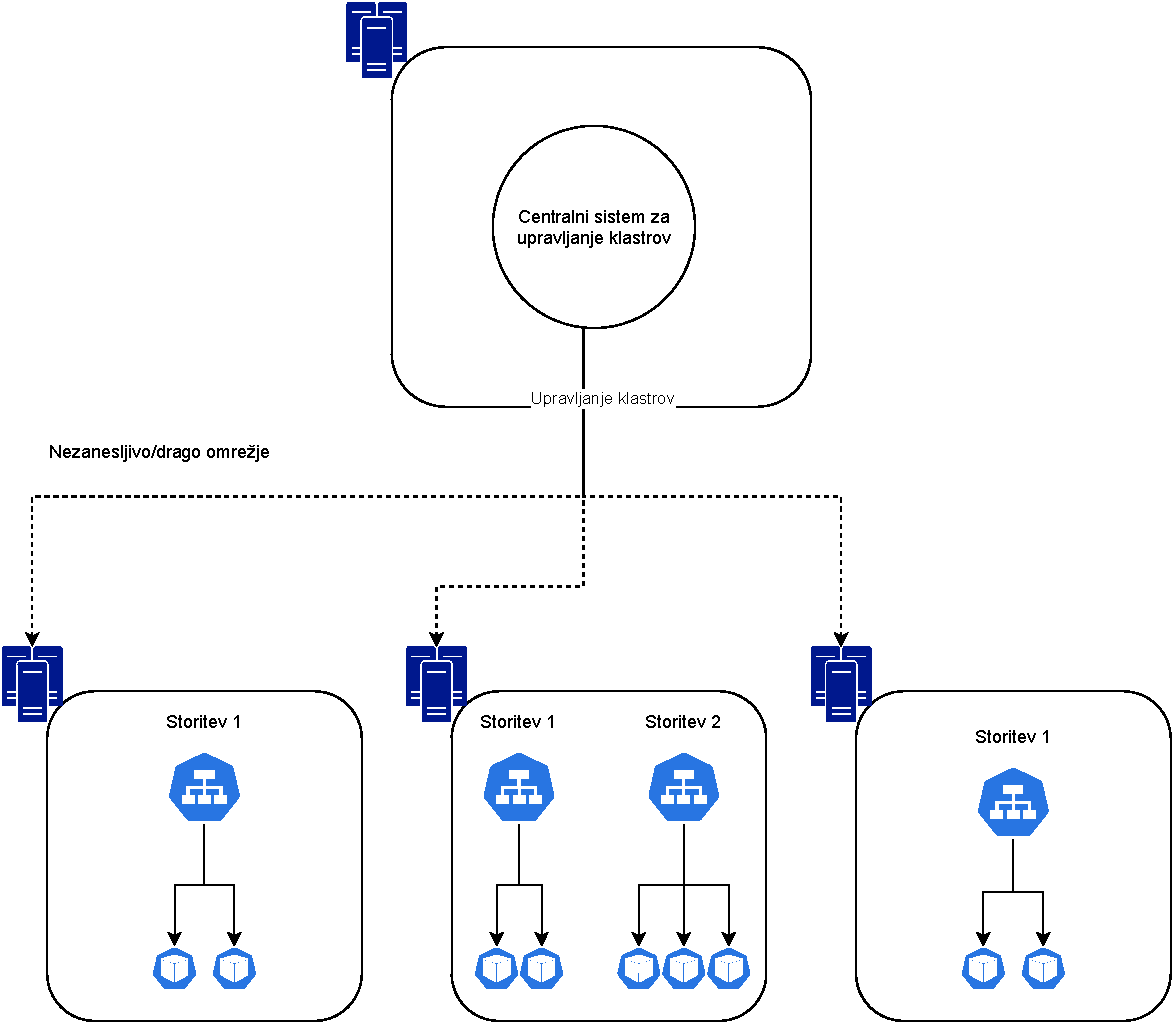
\includegraphics[width=1.0\textwidth]{images/upravljanje-robnih-gruc.pdf}
\end{center}
\caption{Primer izoliranih aplikacij.}
\label{problem-prevelike-latence}
\end{figure}

Nam pa KubeFed omogoča še eno lepo možnost s svojo strukturo in lahko s svojim kontrolerjem in KubeFed vmesnikom implementiramo še dodatne funkcionalnosti kot so razporejanje obremenjenosti med lokalnimi strežniki in po potrebi povečujemo število primerkov ali pa kar razporejamo opravila s Kubernetes Job objekti.

Z zelo preprosto integracijo v Kubernetes nam KubeFed vmesnik tu res omogoča zelo preprosto implementacijo katerekoli naše rešitve.
\section{Sinhronizacija podatkov}
V primeru gruč na robu oblaka bomo sinhronizacijo verjetno implementirali sami, saj le mi vemo kakšen problem rešujemo in zakaj smo sploh postavljali gruče na robu oblaka.

Za primer vzemimo hipotetični varnostni sistem korporacije, ki centralno spremlja varnost v posameznih podružnicah.
Sistem ima eno nadzorno kamero pri vhodu v vsako podružnico.
Želimo, da naša kamera prepoznava obraze in na podlagi tega dovoljuje zaposlenim vstop.
V našem centralnem sistemu pa želimo, hraniti seznam vstopov.
En način reševanja tega problema je z gručami na robu oblaka.
V vsako podružnico bi postavili gručo rač\-un\-al\-ni\-kov Raspberry PI, ki so dovolj zmogljivi, da obdelujejo posnetke kamer in prepoznavajo obraze.
Če posnetke obdelujemo lokalno, se izognemo pošiljanju veliki količini podatkov na centralne strežnike, posledično pa bo hitrejše tudi preverjanje zaposlenih.
Tako bi na centralni strežnik pošiljali samo številko zaposlenega in čas vstopa.
Takšen pristop bi prišel še toliko bolj do izraza, če imajo podružnice dostop do interneta samo prek dragega mobilnega omrežja, kjer lahko z zmanjšanjem prometa zelo zmanjšamo tudi stroške podjetja.
Vse te gruče na podružnicah bi imele zelo podobno strukturo in jih je smiselno centralo upravljati s kakšnim sistemom za povezovanje. 
Tu bi lahko uporabili KubeFed ali GitOps pristop.
Pošiljanje podatkov na centrali strežnik pa bi morali napisati sami in ga vgraditi v naš program za prepoznavo obrazov.
\chapter{Sklepne ugotovitve}
V diplomskem delu smo si pogledali teoretično ozadje povezovanja več rač\-un\-al\-ni\-ških gruč in osnove Kubernetesa.
Predstavljenih je bilo tudi nekaj popularnih orodij za delo z več Kubernetes gručami.
V praktičnem delu pa smo se posvetili predvsem reševanju pogostih problemov v industriji, ki zahtevajo povezovanje več gruč.
Zato pa je bilo potrebo postaviti tudi ustrezno okolje za preizkušanje naših rešitev.

Z razvojem Kubernetesa se je razvilo tudi zelo veliko odprtokodnih orodij, ki omogočajo lažje upravljanje in povezovanje več gruč.
Tako so napredne tehnologije prišle v roke širšemu krogu ljudi in jim omogočajo preprostejše reševanje težav.
Kubernetes pa je s standardizacijo orkestracije zelo olajšal tudi možnost gostovanja aplikacije pri več različnih oblačnih ponudnikih, kjer se zopet pojavi problem povezovanja več gruč.

Področje orkestracije in povezovanja gruč se bo še zelo razvijalo in tema bo zagotovo zahtevala še veliko diplomskih del.

\newpage %dodaj po potrebi, da bo številka strani za Literaturo v Kazalu pravilna!
\newpage %dodaj po potrebi, da bo številka strani za Literaturo v Kazalu pravilna!
\newpage %dodaj po potrebi, da bo številka strani za Literaturo v Kazalu pravilna!
\newpage %dodaj po potrebi, da bo številka strani za Literaturo v Kazalu pravilna!
\ \\
\clearpage
\addcontentsline{toc}{chapter}{Literatura}
\bibliographystyle{plain}
\bibliography{literatura}
\end{document}
